\documentclass[titlepage]{article}
\usepackage[ukrainian]{babel}
\usepackage{listings}
\usepackage{amsmath}
\usepackage{fontspec}
\setmainfont{Times New Roman}
\usepackage{setspace}
\usepackage{fancyhdr}
\usepackage{titling}
\usepackage[a4paper, top = 20mm, bottom = 20mm, left = 25mm, right = 15mm]{geometry}
\usepackage{graphicx}

\lstset{
	basicstyle=\large,
	breaklines = true,
	language = matlab,
	breakatwhitespace = true,
	numbers = left,
	numberstyle = \tiny,
	columns = flexible,
	frame=tb,
	tabsize=4
}

\makeatletter
\renewcommand\normalsize{%
\@setfontsize\normalsize{14pt}{15pt}}
\makeatother

\preauthor{\begin{flushright}}
\postauthor{\end{flushright}}

\fancypagestyle{empty}{%
	\renewcommand{\headrulewidth}{0pt}
	\cfoot{\normalsize2016}
	\chead{\uppercase{київський національний університет імені тараса шевченка}}
}


\begin{document}

\title{\normalsize Лабораторна робота \textnumero 2}
\author{\vspace{5cm}Виконав: \protect\\ студент 4-го курсу \protect\\ спеціальність Математика \protect\\ Шатохін Михайло}
\date{}
\maketitle
\section{Постановка задачі}
Необхідно розв'язати нелінійну систему рівнянь
\[
\begin{cases}
&\phi(y_1) = \gamma_1,\\
&\frac{y_{i-1} - 2y_i + y_{i+1}}{h^2}-p(x_i)y_i=-f(x_i, y_i), \quad i=\overline{2,n-1},\\
&\psi(y_n)=\gamma_2,
\end{cases}
\]
використовуючи ітераційний метод Ньютона та метод немонотонної прогонки. Введено позначення:
\begin{description}
\item $a=0, b = 1;$
\item $x_i = a+(i-1)h, i=\overline{1,n}; h=\frac{b-a}{n-1}, n=101;$
\item $y$-вектор;
\item $\phi(t)=t^g+cos(t+k), \gamma_1=1, \psi(t)=t^3+\frac{cos(t-k)^2}{k},\gamma_2=d;$
\item $p(t)=(t-a)^g(b-t), f(t,v)=exp(-t+v)-tv;$
\item $k = 21$ --- номер за списком студента в группі;
\item $g = 1$ --- номер группи;
\item $d = 7$ --- день народження студента;
\end{description}
\section{Опис алгоритму}
Враховуючи методичні вказівки до розв'язання, спочатку знаходимо розв'язок першого та останнього рівнянь, далі лінійно апроксимуємо значення в проміжних точках, що використовуємо як початкове наближення для багатовимірного методу Ньютона, який відомий також як метод лінеаризації.

Метод Ньютона в даному випадку застосовується таким чином: нехай необхідно розв'язати рівняння $F(\overline{y}) = 0$. Тоді його можна по аналогії з одновимірним випадком лінеарізувати та отримати $F(\overline{\xi}) = grad(F)(\overline{y}-\overline{\xi})$, де $F(\overline{\xi})=0$, що дає відповідний ітераційний метод: $F(x_{n}) = grad(F)(x_{n+1} - x_n)$. В даному випадку $F(y) = \frac{y_{i-1} - 2y_i + y_{i+1}}{h^2}-p(x_i)y_i+f(x_i, y_i)$. Враховуючи, що розбиття $\{x_i\}$ не залежить від номеру кроку, можна виділити лінійну частину F.
\section{Практична реалізація}
У функції main відбувається завантаження параметрів, виклик основних функції алгоритму та демонстрація отриманого результату.
\lstinputlisting[title=main.m, language=octave]{./main.m}
Функція Diff --- допоміжна, створена для пошуку градієнту векторної функції.
\lstinputlisting[title=Diff.m, language=octave]{./Diff.m}
У функції Solve розв'язується тридіагональна система лінійних рівнянь методом немонотонної прогонки. Для забезпечення універсальності вона також може\\ розв'язувати інші системи, проте це викликає відповідне попередження.
\lstinputlisting[title=Solve.m, language=octave]{./Solve.m}
У функції Newton реалізовані одновимірний метод Ньютона та метод лінеаризації. У випадку, якщо з'являється підозра на існування локального мінімуму (тобто, якщо похідна рівна нулю або градієнт має вироджений), то функція повертає попередження.
\lstinputlisting[title=Newton.m, language=octave]{./Newton.m}
Параметри задачі задані у файлі params.mat. Тут представлені у вигляді, що зрозумілий людині.
\lstinputlisting[title=params.mat, language=octave]{./params.mat}
\newpage
В результаті виконання програми отримується такий результат:
\lstinputlisting[title=output.txt, language=octave]{./output.txt}
Та графік розв'язку:
\begin{figure}[h]
\hspace{-1.5cm}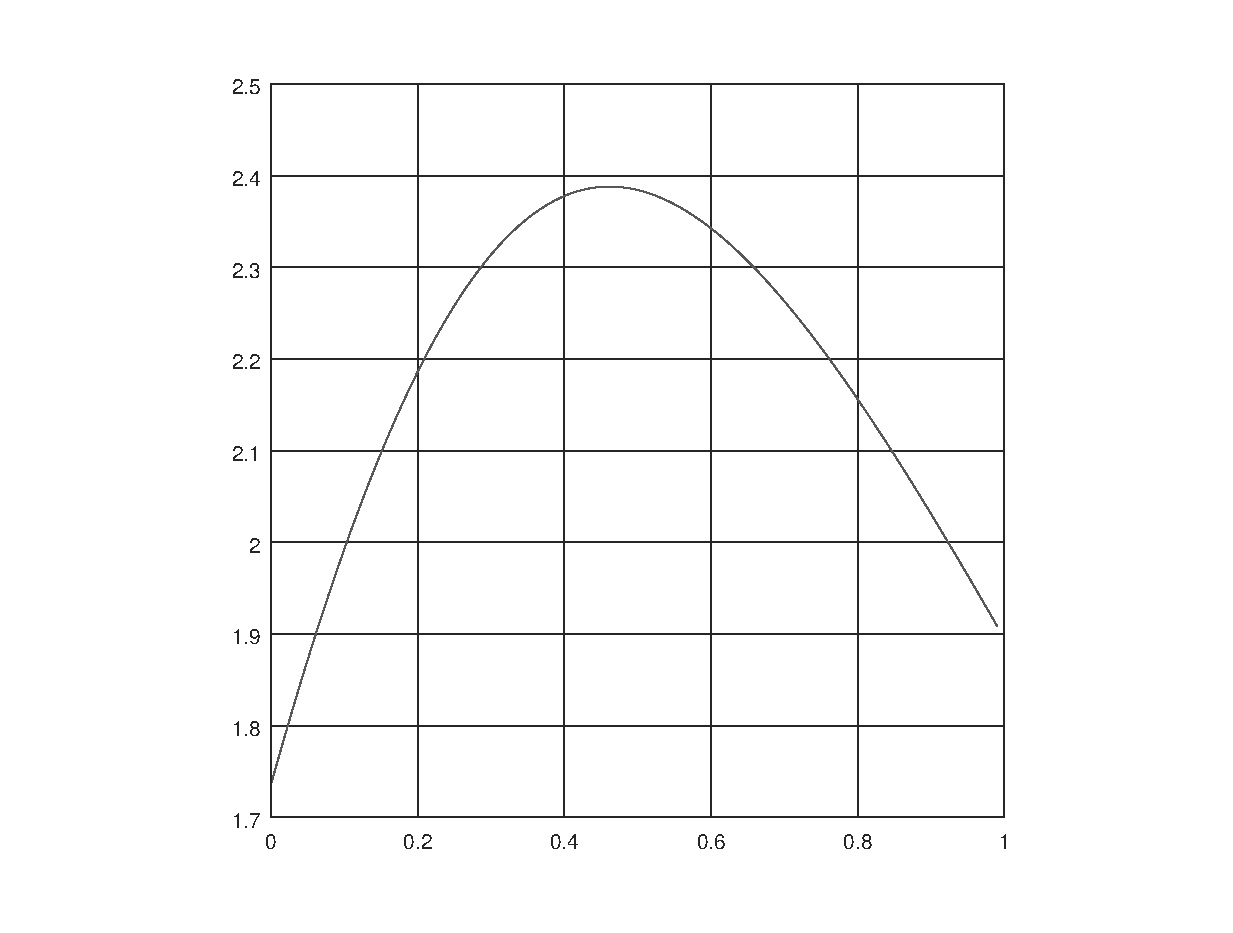
\includegraphics{result.eps}
\end{figure}
\end{document}